

The system is designed as two complementary components:

\begin{enumerate}
    \item A corpus profiling tool, which produces a metadata-only description of the corpus as a multivariate distribution;
    \item A targeted retrieval tool, that attempts to produce a corpus with the same distribution.
\end{enumerate}



\section{Profiling}
The process of constructing a corpus description may be started either from a seed corpus, or from direct user design.

\begin{figure}[h]
    \centering
    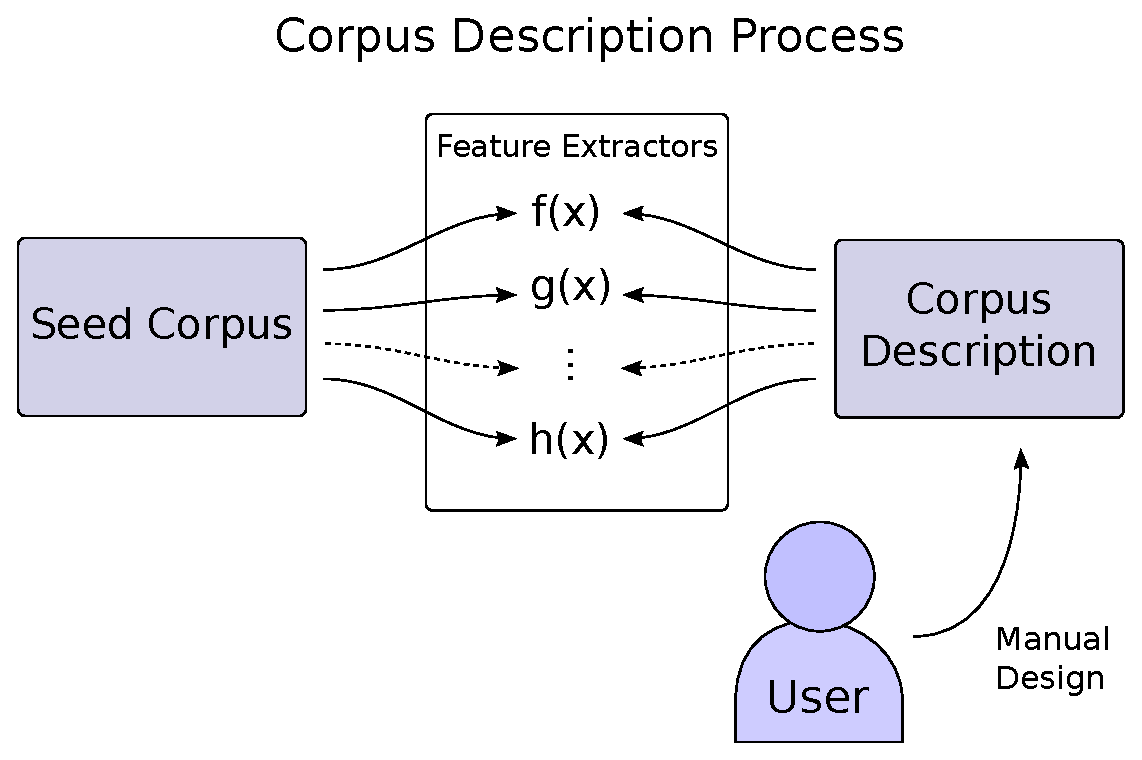
\includegraphics[width=0.8\textwidth]{rebuilding/profiling}
    \caption{Creation of a corpus description}
    \label{fig:rebuilding:profiling}
\end{figure}


The process of building a corpus description is outlined in~\ref{fig:rebuilding:profiling}.  For direct use, the user would specify their salient dimensions, and the distribution for each.  This is essentially a description of the sampling policy---where variables are discrete and nominal (such as genre labels), this would take the form of a table with desired proportions against each.  Where variables are continuous, a probability density function is defined.  Note that this method does not, without prohibitive complexity, allow for specification of interactions between variables\td{return to this and comment on it later}.

Profiling through the use of a `seed' corpus begins with specifications of the salient dimensions, the data for which are then read from the seed (by $f()$ and $g()$ functions in the figure).  As each document is read, the corpus description may contain information not only on marginal distributions for each variable, but also the effects of conditioning on one or more value.

Note that, whichever method is used, this stage is merely a metadata description task.  The corpus description document itself contains no more information than the metadata of the corpora from which is it built---indeed, where all variables are both external and nominal, this reduces to a simple table of frequencies for each desired value.  

Those specifying variables to describe must, as with all sampling, be mindful of their potential systematic correlations with variables of interest to any given research question.  The value of this approach is in documentation---it is possible for a researcher to eyeball the variables (and potentially their distributions) and determine whether or not a corpus is correctly conditioned for use inferring about a given variable.  This cannot be said for bootstrapping systems that use internal variables, which seek to copy corpus contents at the risk of varying their metadata.


% ---

\section{Retrieval}
Retrieval in accordance with the complex distributions specified in a corpus description is challenging in two ways:

\begin{itemize}
    \item Samples must be taken from the corpus description in accordance with a complex empirically-determined distribution;
    \item Any combination of variables sampled from the distribution must then be sought based on its metadata alone.
\end{itemize}

The former of these is difficult because many seed corpora may lack sufficient data to specify their distributions, and because of the high dimensionality of the distributions in question.  These issues may be addressed using techniques such as Gibbs, slice, or rejection sampling.  



\subsection{Resampling}

\td{cite this}
\begin{figure}[h]
    \centering
    \includegraphics[width=0.8\textwidth]{rebuilding/resampling}
    \caption{Resampling the corpus using MCMC methods}
    \label{fig:rebuilding:resampling}
\end{figure}



Resampling from the original corpus produces a `prototype' document, which has values of metadata fields that, over time, hold the same distribution as those in the seed corpus.

The process of constructing a new corpus is one of continually producing these `prototypes' conditional on the values of metadata already sampled, and then retrieving texts matching each.

To perform this resampling, we must be able to sample from a distribution proportional to that of each variable conditional on all of the others, requiring that the corpus description contains information on interactions between values.  As such it is only possible if the original corpus description document contains this information, something that is only practically a product of describing an existing set of documents (as manually filling in the values would be prohibitively expensive).


There are a number of methods by which this prototype document may be selected.  For the purposes of this study, two were implemented:

\begin{itemize}
    \item Simple selection from marginals.  This is the best case possible where a corpus lacks interaction information, and follows the joint distribution of the metadata properties across the whole corpus.  Despite its relative simplicity it may be suitable for some corpus designs, and is analogous to the BNC's balancing of spoken corpora \td{check this, cite the page where they describe their balancing}.
    \item Full conditional selection.  This is implemented by selecting a random sequence of metadata types, and then conditioning on a value drawn from the distribution of that type conditional on the values selected for those previous to it.
\end{itemize}

\til{Does this need the algorithm for both here?  It's terribly simple}

The former of these, whilst faster and simpler, will fail to take into account any interactions between metadata and is included since it is the only method capable of running on a very simply specified corpus description.  The experiments in this thesis use full conditional selection, as they have the luxury of using a corpus description built from a full seed corpus.



\subsection{Seeking the Prototype}
The main practical problem of sampling according to the original corpus' distribution is now framed as an information retrieval task.

This retrieval task is challenging on its own, but errors in performing it have specific ramifications for this sampling process:

\begin{itemizeTitle}
    \item[Dimensionality]As the number of metadata properties in the prototype increases, the search space from which a document must be selected increases exponentially\footnote{Or, strictly, somewhere between linearly and exponentially, if the metadata properties are not truly orthogonal}.  This has severe ramifications for rejection sampling techniques, which become intractable where the ratio of the search space to the area under the target distribution is high.

    \item[Selection of dimensions]Metadata types are selected for research reasons and do not necessarily correspond easily to existing online indexes or retrieval methods.  This means that even specifically seeking a document with one value of metadata may be a challenging task.

    \item[Error in selection]In part because of the above point, documents retrieved are unlikely to be a perfect match against the prototype.  Errors in multivariate selection will follow the population distribution conditional on those metadata values being sought: something that will introduce systematic (yet measurable) bias in the dataset\footnote{The one, extremely unlikely, exception to this is if the population distribution happens to be the same as the target.}.
\end{itemizeTitle}

The retrieval of a prototype, then, is limited to approaches that take into account not only the value of a metadata property to be sought, but also the nature of the source (in this case the internet) and any interactions that are likely to expand the search space to intractable proportions.  It should, of course, also minimise error in selection.


\begin{figure}[h]
    \centering
    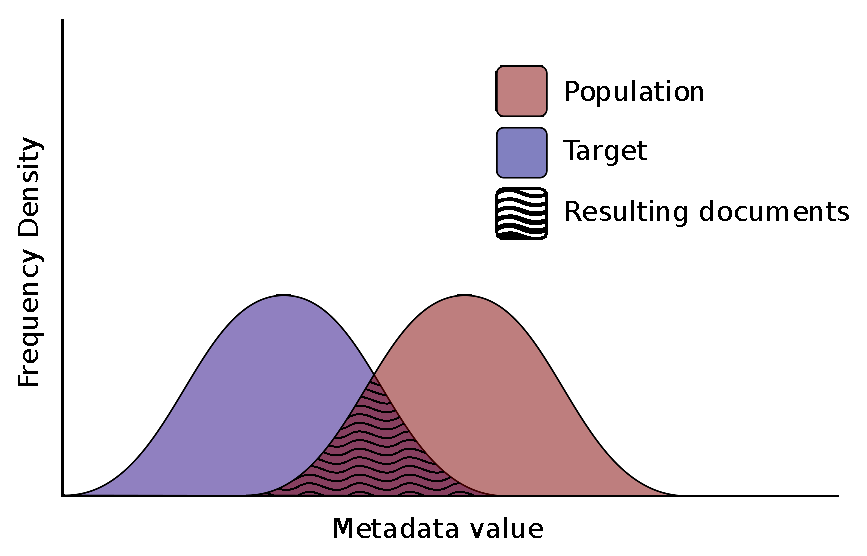
\includegraphics[width=0.8\textwidth]{rebuilding/population-bias}
    \caption{The influence of a biased population distribution on metadata selection}
    \label{fig:rebuilding:population-bias}
\end{figure}


In such a case that the retrieved document is a perfect match to the prototype, the output set of documents will converge to the target distribution.  If it is imperfect but randomly so, there will be an increase in variance in the output distribution.  If it is imperfect and the population is biased (or, in the worst case, does not overlap even slightly with the target), then the results will converge to a distribution with bias following the population distribution.  On Figure~\ref{fig:rebuilding:population-bias}, we rely on the black distribution falling within the red one.

The last of these is the product of an attempt to do something fundamentally impossible: the design of the system is such that this bias is measurable (and may thus be seen to be above some subjective threshold) rather than that it is eliminated for every scenario.  This bias is also evident in existing bootstrapping tools such as BootCaT\td{cite}, however, they seek a looser form of coupling between input and output distributions so this bias often goes un-noticed (or, perhaps, desired\footnote{The comparison of distribution of seed terms to resultant type frequencies yields information about the search method and population, though these are conflated in the process}).

Instead of sampling a corpus \textsl{of} the web, we are sampling one \textsl{from} it, on assumption that the web is already a poorly-indexed supercorpus of documents that are diverse enough to satisfy the majority of research questions.  In terms of Figure~\ref{fig:rebuilding:population-bias}, we assume that the distribution in red has a very high variance (not just in one dimension as illustrated, but also in interaction with other metadata.  Clearly, the case in which this assumption is least strong is the replication of web corpora, and it is perhaps most strong for speech or other particularly specialist sources such as medical notes.

% ---
\paragraph{}

There are multiple possible approaches to this retrieval task, which mirror the web corpus building approaches of searching and sorting.  Though only one was selected for implementation, a few are provided here as counterparts to the conventional bootstrap approach, and to serve as suggestions for further research.

\til{
 * Search for keywords, then take documents on trust
 * Search as seeds, spider, sort fringe by heuristics
 * Scrape links from a web directory or other specific site (i.e. news)
 * Ask people using AMT


 ---
 * Break into dimensions, search, use rejection sampling
 * Select a subcorpus from the target, break into dimensions, search/spider, use Viterbi to balance biases
 * Feedback from output corpus to subtract from target corpus (sample prototype from difference)
 * Send to AMT for manual selection of a document
 (* Use PCA to derive similarity score)
}






%
%Resampling according to multivariate distributions is possible using Gibbs or slice sampling, both of which are MCMC techniques---the `output' distribution of prototype metadata will iteratively approach the distribution of input data.
%
%This process is nonparametric, and thus able to accept arbitrary empirical input distributions and arbitrary modifications thereto.  This allows us to arbitrarily boost the sampling probability of a given category, or to ensure that variables with hitherto-unseen values are considered contributory to the output corpus.
%
%Gibbs sampling is also commonly used to infer the posterior distribution of individual variables by fixing the values of the input distributions.  Though beyond the scope of this thesis, it would be possible to use this technique to fix input variables and identify the distribution of metadata values also described in the corpus description document.  This technique would be highly sensitive to the bias of the retrieval mechanism, and would require a particularly large seed corpus to operate meaningfully.
%

\til{
Theoretically speaking, the corpus is reconstructed as a distribution of all internal variables on the document, conditional on the values in the metadata.  So long as the retrieval engine can find documents fitting the distribution of input data, the output data will conform to the posterior distribution of word frequencies (or any other internal property one wishes to reason about).

Separation of the latent (internal) variables into a block is consistent with a 'block gibbs sampler'.  Ignoring them as a block is consistent with a 'collapsed gibbs sampler'.

% This is awesome: http://www.people.fas.harvard.edu/~plam/teaching/methods/mcmc/mcmc_print.pdf
}


\til{ Describe gibbs formally, and compare slice to it.  Describe the process of resampling from the output using the input distribution. }









